\chapter{End of chapter exercise solutions}
\label{eoceSolutions}



%_______________
\eocesolch{Introduction to data}



%_______________
\begin{multicols}{2}

% 1

\eocesol{(a)~Treatment: $10/43 = 0.23 \rightarrow 23\%$. \\
Control: $2/46 = 0.04 \rightarrow 4\%$. 
(b)~There is a 19\% difference between the pain reduction rates in the two 
groups. At first glance, it appears patients in the treatment group are more 
likely to experience pain reduction from the acupuncture treatment. 
(c)~Answers may vary but should be sensible. Two possible answers: $^1$Though 
the groups' difference is big, I'm skeptical the results show a real difference 
and think this might be due to chance. $^2$The difference in these rates looks 
pretty big, so I suspect acupuncture is having a positive impact on pain.}

% 3

\eocesol{(a)~143,196 eligible study subjects born in Southern California between 1989 
and 1993. 
(b)~Measurements of carbon monoxide, nitrogen dioxide, ozone, and particulate 
matter less than 10$\mu g/m^3$ (PM$_{10}$) collected at air-quality-monitoring 
stations as well as length of gestation. Continuous numerical variables. 
(c)~``Is there an association between air pollution 
exposure and preterm births?"}

% 5

\eocesol{(a)~160 children.
(b)~Age (numerical, continuous), sex (categorical), whether they were an only child or 
not (categorical).
(c)~Research question: ``Does explicitly telling children not to cheat affect their 
likelihood to cheat?"}

% 7

\eocesol{(a)~$50 \times 3 = 150$. 
(b)~Four continuous numerical variables: sepal length, sepal width, petal length, and petal width. 
(c)~One categorical variable, species, with three levels: \emph{setosa}, \emph{versicolor}, and \emph{virginica}.}

% 9

\eocesol{(a)~Population: all births, sample: 143,196 births between 1989 and 1993 in 
Southern California. 
(b)~If births in this time span at the geography can be considered to be 
representative of all births, then the results are generalizable to the 
population of Southern California. However, since the study is observational 
the findings cannot be used to establish causal relationships.}

% 11

\eocesol{(a)~Population: all asthma patients aged 18-69 who rely on medication for 
asthma treatment. Sample: 600 such patients.
(b)~If the patients in this sample, who are likely not randomly sampled, can 
be considered to be representative of all asthma patients aged 18-69 who rely 
on medication for asthma treatment, then the results are generalizable to the 
population defined above. Additionally, since the study is experimental, the 
findings can be used to establish causal relationships.}

% 13

\eocesol{(a)~Observation.
(b)~Variable.
(c)~Sample statistic (mean).
(d)~Population parameter (mean).}


\end{multicols}
\textC{\newpage}
\begin{multicols}{2}

% 15

\eocesol{(a)~Explanatory: number of study hours per week. Response: GPA.
(b)~Somewhat weak positive relationship with data becoming more sparse as the 
number of study hours increases. One responded reported a GPA above 4.0, which 
is clearly a data error. There are a few respondents who reported unusually 
high study hours (60 and 70 hours/week). Variability in GPA is much higher for 
students who study less than those who study more, which might be due to the 
fact that there aren't many respondents who reported studying higher hours.
(c)~Observational.
(d)~Since observational, cannot infer causation.}

% 17

\eocesol{(a)~Observational.
(b)~Use stratified sampling to randomly sample a fixed number of students, 
say 10, from each section for a total sample size of 40 students.}

% 19

\eocesol{(a)~Positive, non-linear, somewhat strong. Countries in which a higher 
percentage of the population have access to the internet also tend to have 
higher average life expectancies, however rise in life expectancy trails 
off before around 80 years old.
(b)~Observational.
(c)~Wealth: countries with individuals who can widely afford the internet 
can probably also afford basic medical care. (Note: Answers may vary.)}

% 21

\eocesol{(a)~The cases are 200 randomly sampled men and women.
(b)~The response variable is attitude towards a fictional microwave oven.
(c)~The explanatory variable is dispositional attitude.
(d)~Yes, the cases are sampled randomly.
(e)~This is an observational study since there is no random assignment to 
treatments.
(f)~No, we cannot establish a causal link between the explanatory and response 
variables since the study is observational.
(g)~Yes, the results of the study can be generalized to the population at 
large since the sample is random.}

% 23

\eocesol{(a)~Non-responders may have a different response to this question, e.g. 
parents who returned the surveys likely don't have difficulty spending time 
with their children.
(b)~It is unlikely that the women who were reached at the same address 3 years 
later are a random sample. These missing responders are probably renters 
(as opposed to homeowners) which means that they might be in a lower socio-
economic status than the respondents.
(c)~There is no control group in this study, this is an observational study, 
and there may be confounding variables, e.g. these people may go running 
because they are generally healthier and/or do other exercises.}

% 25

\eocesol{(a)~Simple random sample. Non-response bias, if only those people who have 
strong opinions about the survey responds his sample may not be representative 
of the population.
(b)~Convenience sample. Under coverage bias, his sample may not be 
representative of the population since it consists only of his friends. It is 
also possible that the study will have non-response bias if some choose to not 
bring back the survey.
(c)~Convenience sample. This will have a similar issues to handing out surveys 
to friends.
(d)~Multi-stage sampling. If the classes are similar to each other with 
respect to student composition this approach should not introduce much bias, 
other than potential non-response bias.}

% 27

\eocesol{No, students were not randomly sampled (voluntary sample) and the sample only 
contains college students at a university in Ontario.}

% 29

\eocesol{(a)~Exam performance.
(b)~Light level: fluorescent overhead lighting, yellow overhead lighting, no overhead 
lighting (only desk lamps).
(c)~Sex: man, woman.}

% 31

\eocesol{(a)~Exam performance.
(b)~Light level (overhead lighting, yellow overhead lighting, no overhead lighting) and 
noise level (no noise, construction noise, and human chatter noise).
(c)~Sex.}

% 33

\eocesol{Need randomization and blinding. One possible outline: (1) Prepare two cups for each 
participant, one containing regular Coke and the other containing Diet Coke. Make sure 
the cups are identical and contain equal amounts of soda. Label the cups A (regular) and 
B (diet). (Be sure to randomize A and B for each trial!) (2) Give each participant the 
two cups, one cup at a time, in random order, and ask the participant to record a value 
that indicates how much she liked the beverage.  Be sure that neither the participant nor 
the person handing out the cups knows the identity of the beverage to make this a double-
blind experiment. (Answers may vary.)}


\end{multicols}
\textC{\newpage}
\begin{multicols}{2}


% 35

\eocesol{(a)~Experiment.
(b)~Treatment: 25 grams of chia seeds twice a day, control: placebo. 
(c)~Yes, gender.
(d)~Yes, single blind since the patients were blinded to the treatment 
they received.
(e)~Since this is an experiment, we can make a causal statement. However, since the 
sample is not random, the causal statement cannot be generalized to the population at 
large.}

% 37

\eocesol{(a)~(1) - linear and (3) - nonlinear
(b)~(4) - linear
(c)~(2)}

% 39

\eocesol{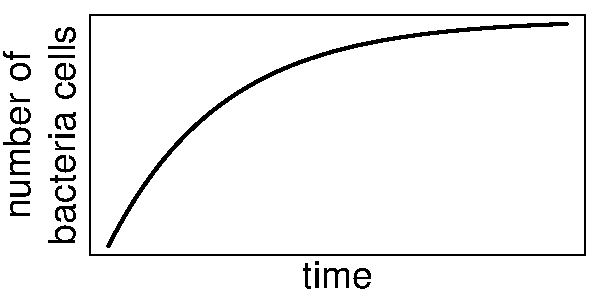
\includegraphics[width = 40mm]{ch_intro_to_data/figures/eoce/reproducing_bacteria/reproducing_bacteria_sketch.pdf}}

% 41

\eocesol{(a)~Population mean, $\mu_{2007} = 52$; sample mean, $\bar{x}_{2008} = 58$.
(b)~Population mean, $\mu_{2001} = 3.37$; sample mean, $\bar{x}_{2012} = 3.59$.}

% 43

\eocesol{Any 10 employees whose average number of days off is between the minimum and the mean 
number of days off for the entire workforce at this plant.}

% 45

\eocesol{(a)~Distribution (2) has a higher mean since $20 > 8$, and a higher standard deviation 
since 20 is much further from the rest of the data than 8.
(b)~Distribution (1) has a higher mean since $-20 > -40$, and distribution (2) has a 
higher standard deviation since -40 is farther away from the rest of the data than -20.
(c)~Distribution (2) has a higher mean since all values in this distribution are higher 
than those in distribution (1), but both distribution have the same standard deviation 
since they are equally variable around their respective means.
(d)Both distributions have the same mean since they're both centered at 300, but 
distribution (2) has a higher standard deviation since the observations are farther from 
the mean than in distribution (1).}

% 47

\eocesol{(a)~Q1 $\approx$ 5, median $\approx$ 15, Q3 $\approx$ 35
(b)~Since the distribution is right skewed, we would expect the mean to be higher than the median.}

% 49

\eocesol{(a)~Between 25 and 30.
(b)~Since the distribution is right skewed the mean is higher than the median.
(c)~Q1: between 15 and 20, Q3: between 35 and 40, IQR: about 20
(d)~Values that are considered to be unusually low or high lie more than 1.5$\times$IQR 
away from the quartiles. Upper fence: Q3 + 1.5 $\times$ IQR =  $37.5 + 1.5 \times 20 = 67.5$; 
Lower fence: Q1 - 1.5 $\times$ IQR =  $17.5 + 1.5 \times 20 =  -12.5$; The lowest AQI 
recorded is not lower than 5 and the highest AQI recorded is not higher than 65, which 
are both within the fences. Therefore none of the days in this sample would be considered 
to have an unusually low or high AQI.}

% 51

\eocesol{The histogram shows that the distribution is bimodal, which is not apparent in the box 
plot. The box plot makes it easy to identify more precise values of observations outside 
of the whiskers.}

% 53

\eocesol{(a)~The distribution of number of pets per household is likely right skewed as there is a natural boundary at 0 and only a few people have many pets. Therefore the center would be best described by the median, and variability would be best described by the IQR.
(b)~The distribution of number of distance to work is likely right skewed as there is a natural boundary at 0 and only a few people live a very long distance from work. Therefore the center would be best described by the median, and variability would be best described by the IQR.
(c)~The distribution of heights of males is likely symmetric. Therefore the center would be best described by the mean, and variability would be best described by the standard deviation.}

% 55

\eocesol{No, we would expect this distribution to be right skewed. There are two reasons 
for this: (1) there is a natural boundary at 0 (it is not possible to watch less 
than 0 hours of TV), (2) the standard deviation of the distribution is very large 
compared to the mean.}

% 57

\eocesol{The statement ``50\% of Facebook users have over 100 friends" means that the median 
number of friends is 100, which is lower than the mean number of friends (190), which 
suggests a right skewed distribution for the number of friends of Facebook users.}


\end{multicols}
\textC{\newpage}
\begin{multicols}{2}


% 59

\eocesol{(a)~The median is a much better measure of the typical amount earned by these 42 
people. The mean is much higher than the income of 40 of the 42 people. This is 
because the mean is an arithmetic average and gets affected by the two extreme observations. The median does not get effected as much since it is robust to 
outliers.
(b)~The IQR  is a much better measure of variability in the amounts earned by nearly 
all of the 42 people. The standard deviation gets affected greatly by the two high 
salaries, but the IQR is robust to these extreme observations.}

% 61

\eocesol{(a)~The distribution is unimodal and symmetric with a mean of about 25 minutes 
and a standard deviation of about 5 minutes. There does not appear to be any 
counties with unusually high or low mean travel times. Since the distribution 
is already unimodal and symmetric, a log transformation is not necessary.
(b)~Answers will vary. There are pockets of longer travel time around DC, 
Southeastern NY, Chicago, Minneapolis, Los Angeles, and many other big cities. 
There is also a large section of shorter average commute times that overlap 
with farmland in the Midwest. Many farmers' homes are adjacent to their 
farmland, so their commute would be 0 minutes, which may explain why the 
average commute time for these counties is relatively low.}

% 63

\eocesol{(a)~We see the order of the categories and the relative frequencies in the bar plot.
(b)~There are no features that are apparent in the pie chart but not in the bar plot.
(c)~We usually prefer to use a bar plot as we can also see the relative frequencies of the categories in this graph.}

% 65

\eocesol{The vertical locations at which the ideological groups break into the Yes, No, 
and Not Sure categories differ, which indicates that likelihood of supporting 
the DREAM act varies by political ideology. This suggests that the two variables 
may be dependent.}

% 67

\eocesol{(a)~(i) False. Instead of comparing counts, we should compare percentages of people in each group who suffered cardiovascular problems.
(ii)~True.
(iii)~False. Association does not imply causation. We cannot infer a causal relationship based on an observational study. (We cannot say changing the drug a person is on affects her risk, which is why part (b) is true. The difference in these statements is subtle.)
(iv)~True.
(b)~Proportion of all patients who had a heart attack: $\frac{7,979}{227,571} \approx 0.035$
(c)~Expected number of heart attacks in the rosiglitazone group if having cardiovascular problems and treatment were independent can be calculated as the number of patients in that group multiplied by the overall cardiovascular problem rate in the study: $67,593 * \frac{7,979}{227,571} \approx 2370$.
(d)~(i)~$H_0$: The treatment and cardiovascular problems are independent. They have no relationship, and the difference in incidence rates between the rosiglitazone and pioglitazone groups is due to chance. \\
$H_A$: The treatment and cardiovascular problems are not independent. The difference in the incidence rates between the rosiglitazone and pioglitazone groups is not due to chance and rosiglitazone is associated with an increased risk of serious cardiovascular problems.
(ii)~A higher number of patients with cardiovascular problems than expected under the assumption of independence would provide support for the alternative hypothesis as this would suggest that rosiglitazone increases the risk of such problems.
(iii)~In the actual study, we observed 2,593 cardiovascular events in the rosiglitazone group. In the 1,000 simulations under the independence model, we observed somewhat less than 2,593 in every single simulation, which suggests that the actual results did not come from the independence model. That is, the variables do not appear to be independent, and we reject the independence model in favor of the alternative. The study's results provide convincing evidence that rosiglitazone is associated with an increased risk of cardiovascular problems.}



%_______________
\end{multicols}


\textC{\newpage}


%_______________
\eocesolch{Probability}



%_______________
\begin{multicols}{2}

% 1

\eocesol{(a)~False. These are independent trials.
(b)~False. There are red face cards.
(c)~True. A card cannot be both a face card and an ace.}

% 3

\eocesol{(a)~10 tosses. Fewer tosses mean more variability in the sample fraction of heads, 
meaning there's a better chance of getting at least 60\% heads.
(b)~100 tosses. More flips means the observed proportion of heads would often be 
closer to the average, 0.50, and therefore also above 0.40.
(c)~100 tosses. With more flips, the observed proportion of heads would often be 
closer to the average, 0.50.
(d)~10 tosses. Fewer flips would increase variability in the fraction of tosses 
that are heads.}

% 5

\eocesol{(a)~$0.5^{10}$ = 0.00098.
(b)~$0.5^{10}$ = 0.00098.
(c)~$P$(at least one tails) = $1 - P$(no tails) = $1 - (0.5^{10}) \approx 1 - 0.001 = 0.999$.}

% 7

\eocesol{(a)~No, there are voters who are both independent and swing voters.
(b)~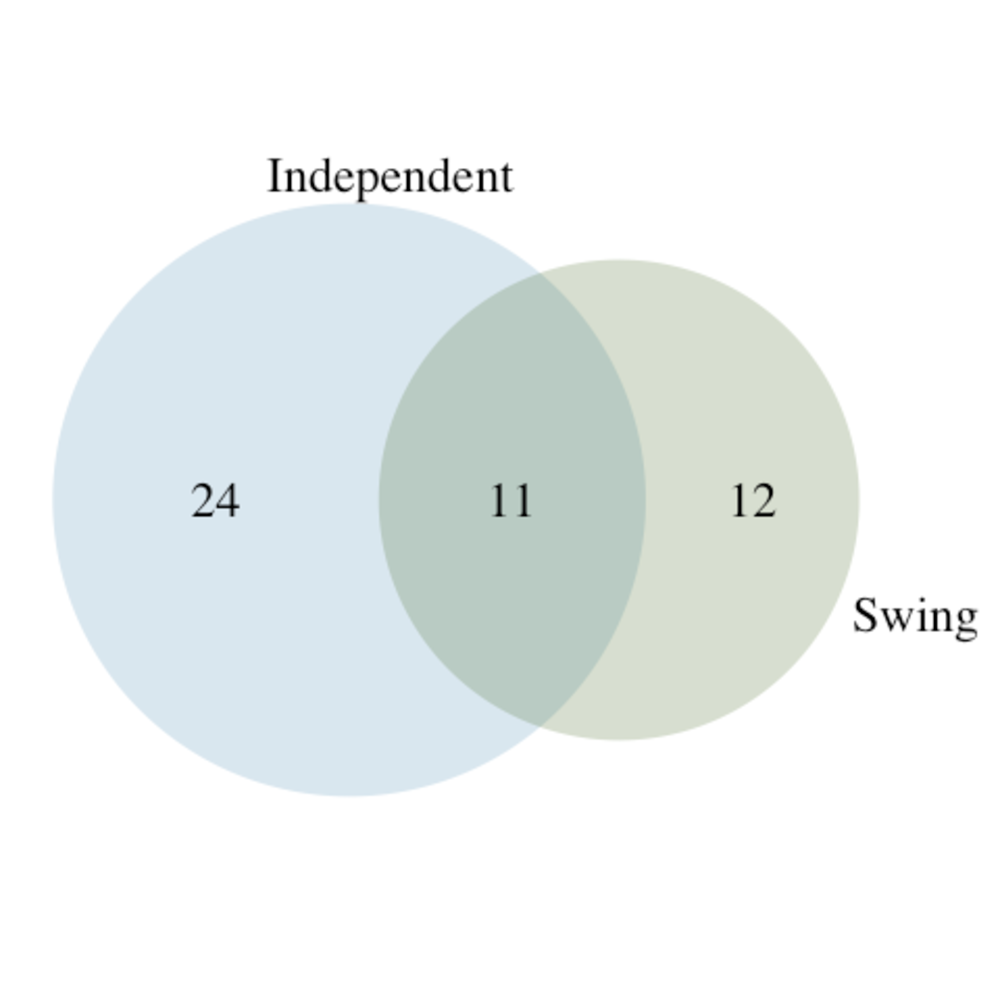
\includegraphics[width=40mm]{ch_probability/figures/eoce/swing_voters/swing_voters.pdf}
(c)~Each Independent voter is either a swing voter or not. Since 35\% of voters 
are Independents and 11\% are both Independent and swing voters, the other 24\% 
must not be swing voters.
(d)~0.47,
(e)~0.53.
(f)~P(Independent) $\times$ P(swing) = $0.35\times0.23 = 0.08$, which 
does not equal P(Independent and swing) = 0.11, so the events are dependent.}

% 9

\eocesol{(a)~If the class is not graded on a curve, they are independent. If graded on a 
curve, then neither independent nor disjoint (unless the instructor will only give 
one A, which is a situation we will ignore in parts~(b) and~(c)).
(b)~They are probably not independent: if you study together, your study habits 
would be related, which suggests your course performances are also related.
(c)~No. See the answer to part~(a) when the course is not graded on a curve. More 
generally: if two things are unrelated (independent), then one occurring does not 
preclude the other from occurring.}

% 11

\eocesol{(a)~$0.16 + 0.09 = 0.25$.
(b)~$0.17 + 0.09 = 0.26$.
(c)~Assuming that the education level of the husband and wife are independent: 
$0.25 \times 0.26 = 0.065$. You might also notice we actually made a second 
assumption: that the decision to get married is unrelated to education level.
(d)~The husband/wife independence assumption is probably not reasonable, because 
people often marry another person with a comparable level of education. We will 
leave it to you to think about whether the second assumption noted in part~(c) is 
reasonable.}

% 13

\eocesol{(a)~Invalid. Sum is greater than 1.
(b)~Valid. Probabilities are between 0 and 1, and they sum to 1. In this class, 
every student gets a C.
(c)~Invalid. Sum is less than 1.
(d)~Invalid. There is a negative probability.
(e)~Valid. Probabilities are between 0 and 1, and they sum to 1.
(f)~Invalid. There is a negative probability.}

% 15

\eocesol{(a)~No, but we could if A and B are independent.
(b-i)~0.21.
(b-ii)~0.79.
(b-iii)~0.3. 
(c)~No, because 0.1 $\ne$ 0.21, where 0.21 was the value computed under 
independence from part~(a).
(d)~0.143.}

% 17

\eocesol{(a)~0.62.
(b)~0.90.
(c)~0.33.
(d)~No, otherwise the final answers of parts (b) and (c) would have been equal.
(e)~0.18.}

% 19

\eocesol{(a)~$162/248 = 0.65$.
(b)~$181/252 = 0.72$.
(c)~Under the assumption of a dating choices being independent of 
hamburger preference, which on the surface seems reasonable: 
$0.65 \times 0.72 = 0.468$.
(d)~$(252 + 6 - 1)/500 = 0.514$.}

% 21

\eocesol{(a) \\
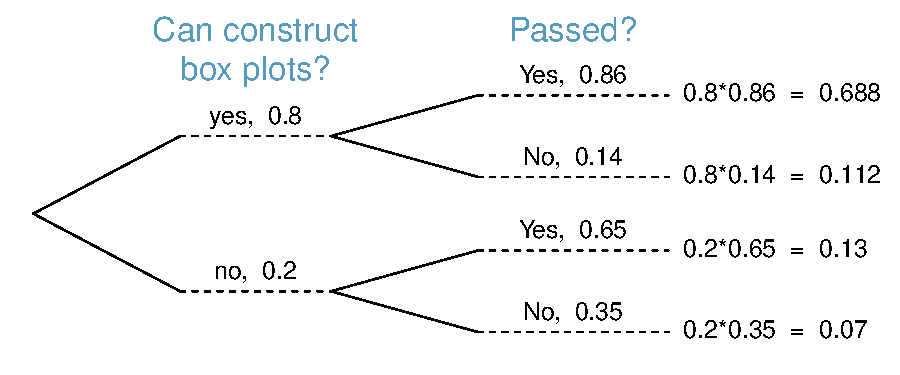
\includegraphics[width=60mm]{ch_probability/figures/eoce/tree_drawing_box_plots/tree_drawing_box_plots} \\
(b)~0.84}


\end{multicols}
\textC{\newpage}
\begin{multicols}{2}


% 23

\eocesol{0.8247. \\
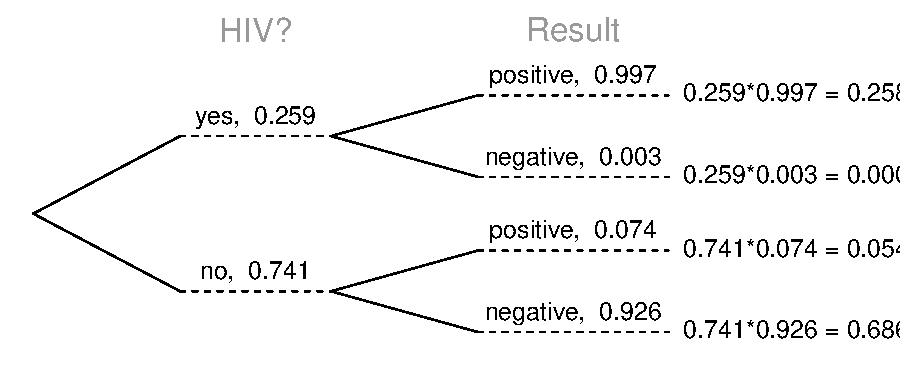
\includegraphics[width=60mm]{ch_probability/figures/eoce/tree_hiv_swaziland/tree_hiv_swaziland.pdf}}

% 25

\eocesol{0.0714. Even when a patient tests positive for lupus, there is only a 7.14\% 
chance that he actually has lupus. House may be right.
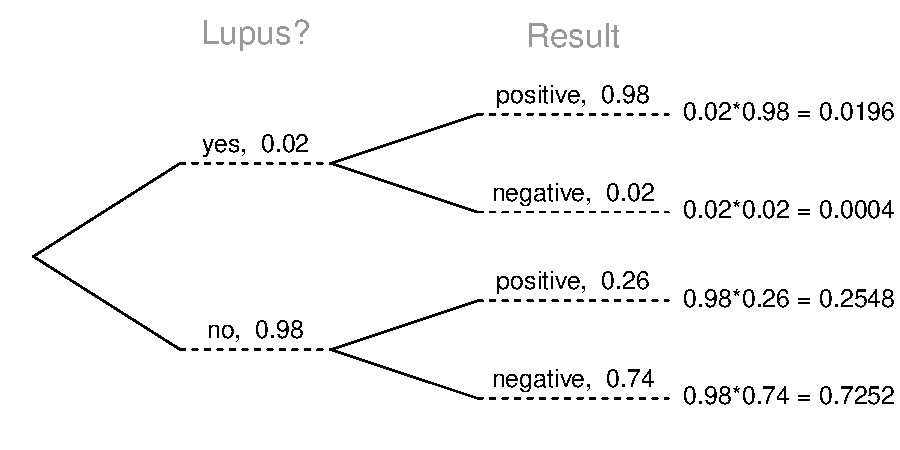
\includegraphics[width=60mm]{ch_probability/figures/eoce/tree_lupus/tree_lupus.pdf}}

% 27

\eocesol{(a)~0.3.
(b)~0.3.
(c)~0.3.
(d)~$0.3\times0.3=0.09$.
(e)~Yes, the population that is being sampled from is identical in each draw.}

% 29

\eocesol{(a)~0.22.
(b)~$3/9 = 0.33$.
(c)~$\frac{3}{10} \times \frac{2}{9} \approx 0.067$.
(d)~No. In this small population of marbles, removing one marble meaningfully 
changes the probability of what might be drawn next.}

% 31

\eocesol{0.0519.}

% 33

\eocesol{(a)~13.
(b)~No, these 27 students are not a random sample from the university's student 
population. For example, it might be argued that the proportion of smokers among 
students who go to the gym at 9 am on a Saturday morning would be lower than the 
proportion of smokers in the university as a whole.}

% 35

\eocesol{(a)~E(X) = 3.59. SD(X) = 3.37.
(b)~E(X) = -1.41. SD(X) = 3.37.
(c)~No, the expected net profit is negative, so on average you expect to lose money.}

% 37

\eocesol{5\% increase in value.}

% 39

\eocesol{E = -0.0526. SD = 0.9986.}

% 41

\eocesol{(a)~E = \$3.90. SD = \$0.34.
(b)~E = \$27.30. SD = \$0.89.}

% 43

\eocesol{Approximate answers are OK. Answers are only estimates based on the sample. 
(a)~$(29+32)/144 = 0.42$.
(b)~$21/144 = 0.15$.
(c)~$(26+12+15)/144 = 0.37$.}



%_______________
\end{multicols}






%_______________
\eocesolch{Distributions of random variables}



%_______________
\begin{multicols}{2}

% 1

\eocesol{(a)~8.85\%.
(b)~6.94\%.
(c)~58.86\%.
(d)~4.56\%. \\
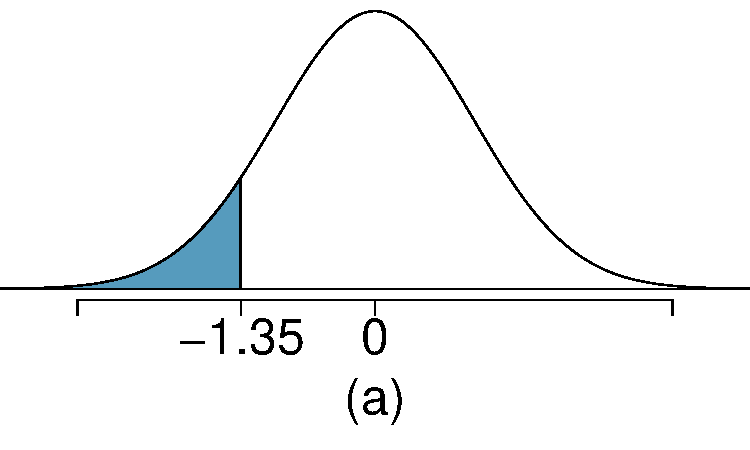
\includegraphics[width=0.23\textwidth]{ch_distributions/figures/eoce/area_under_curve_1/zltNeg}
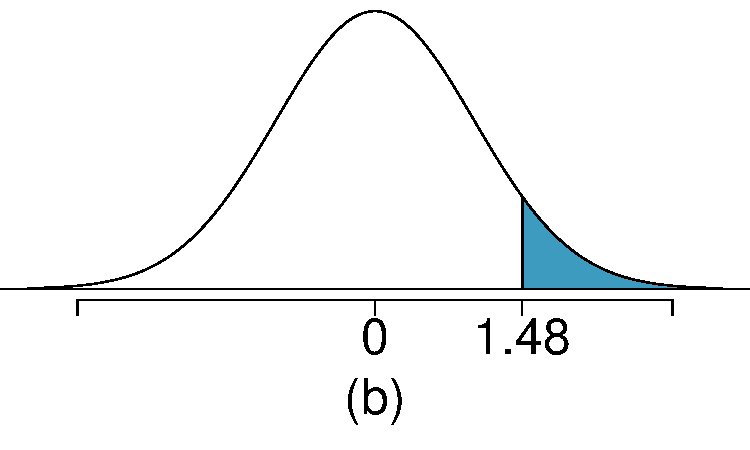
\includegraphics[width=0.23\textwidth]{ch_distributions/figures/eoce/area_under_curve_1/zgtPos}
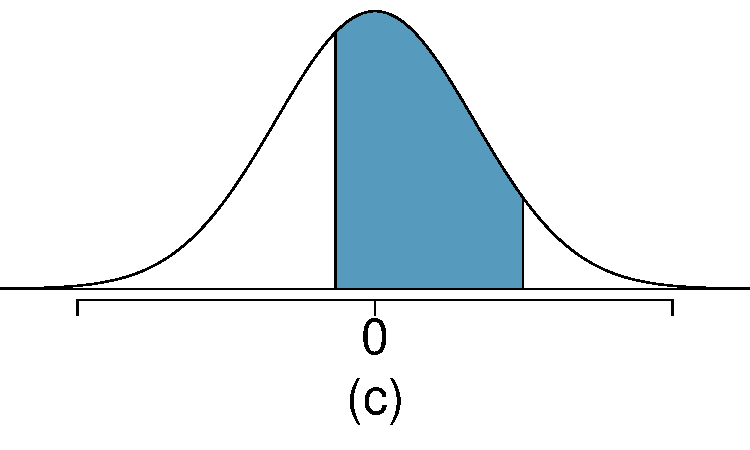
\includegraphics[width=0.23\textwidth]{ch_distributions/figures/eoce/area_under_curve_1/zBet}
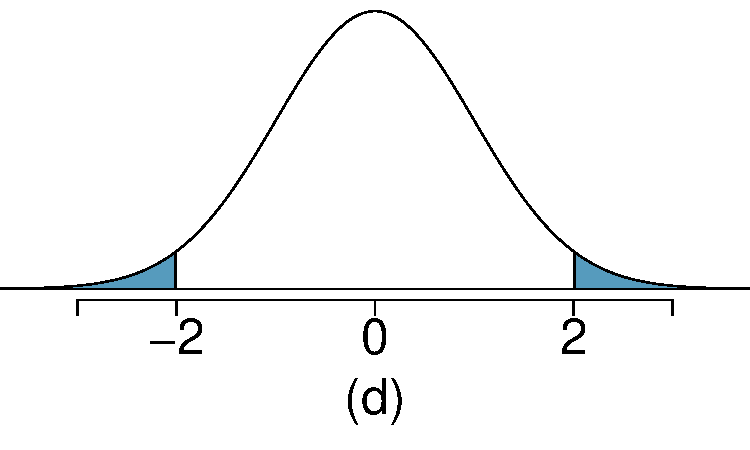
\includegraphics[width=0.23\textwidth]{ch_distributions/figures/eoce/area_under_curve_1/zgtAbs}}

% 3

\eocesol{(a)~Verbal: $N(\mu = 151, \sigma = 7)$, Quant: $N(\mu = 153, \sigma = 7.67)$.
(b)~$Z_{VR} = 1.29$, $Z_{QR} = 0.52$. \\
\includegraphics[width=0.3\textwidth]{ch_distributions/figures/eoce/GRE_intro/GRE_intro.pdf} \\
(c)~She scored 1.29 standard deviations above the mean on the Verbal 
Reasoning section and 0.52 standard deviations above the mean on the 
Quantitative Reasoning section.
(d)~She did better on the Verbal Reasoning section since her Z-score on that 
section was higher.
(e)~$Perc_{VR} = 0.9007 \approx 90\%$, $Perc_{QR} = 0.6990 \approx 70\%$.
(f)~$100\% - 90\% = 10\%$ did better than her on VR, and $100\% - 70\% = 30\%$
 did better than her on QR.
(g)~We cannot compare the raw scores since they are on different scales. 
Comparing her percentile scores is more appropriate when comparing her 
performance to others.
(h)~Answer to part (b) would not change as Z-scores can be calculated for 
distributions that are not normal. However, we could not answer parts~(d)-(f) 
since we cannot use the normal probability table to calculate probabilities 
and percentiles without a normal model.}


\end{multicols}
\textC{\newpage}
\begin{multicols}{2}


% 5

\eocesol{(a)~$Z = 0.84$, which corresponds to approximately 160 on QR.
(b)~$Z = -0.52$, which corresponds to approximately 147 on VR.}

% 7

\eocesol{(a)~$Z=1.2 \to 0.1151$.
(b)~$Z= -1.28 \to 70.6\degree$F or colder.}

% 9

\eocesol{(a)~$N(25, 2.78)$.
(b)~$Z = 1.08 \to 0.1401$.
(c)~The answers are very close because only the units were changed. (The only 
reason why they are a little different is because 28\degree C is 
82.4\degree F, not precisely 83\degree F.)
(c)~Since $IQR = Q3 - Q1$, we first need to find $Q3$ and $Q1$ and take the 
difference between the two. Remember that $Q3$ is the $75^{th}$ and $Q1$ is 
the $25^{th}$ percentile of a distribution. Q1 = 23.13, Q3 = 26.86, IQR = 26.
86 - 23.13 = 3.73.}

% 11

\eocesol{(a)~$Z=0.67$.
(b)~$\mu=\$1650$, $x=\$1800$.
(c)~$0.67 = \frac{1800-1650}{\sigma} \to \sigma=\$223.88$.}

% 13

\eocesol{$Z = 1.56 \to 0.0594$, i.e. 6\%.}

% 15

\eocesol{(a)~$Z=0.73 \to 0.2327$.
(b)~If you are bidding on only one auction and set a low maximum bid price, 
someone will probably outbid you. If you set a high maximum bid price, you 
may win the auction but pay more than is necessary. If bidding on more than 
one auction, and you set your maximum bid price very low, you probably won't 
win any of the auctions. However, if the maximum bid price is even modestly 
high, you are likely to win multiple auctions.
(c)~An answer roughly equal to the 10th percentile would be reasonable. 
Regrettably, no percentile cutoff point guarantees beyond any possible event 
that you win at least one auction. However, you may pick a higher percentile 
if you want to be more sure of winning an auction.
(d)~Answers will vary a little but should correspond to the answer in 
part~(c). We use the 10$^{th}$ percentile: $Z = -1.28 \to \$69.80$.}

% 17

\eocesol{(a)~70\% of the data are within 1 standard deviation of the mean, 95\% are 
within 2 and 100\% are within 3 standard deviations of the mean. Therefore, 
we can say that the data approximately follow the 68-95-99.7\% Rule.
(b)~The distribution is unimodal and symmetric. The superimposed normal 
curve seems to approximate the distribution pretty well. The points on the 
normal probability plot also seem to follow a straight line. There is one 
possible outlier on the lower end that is apparent in both graphs, but it is 
not too extreme. We can say that the distribution is nearly normal.}

% 19

\eocesol{(a)~No. The cards are not independent. For example, if the first card is an 
ace of clubs, that implies the second card cannot be an ace of clubs. 
Additionally, there are many possible categories, which would need to be 
simplified.
(b)~No. There are six events under consideration. The Bernoulli distribution 
allows for only two events or categories. Note that rolling a die could be a 
Bernoulli trial if we simply to two events, e.g. rolling a 6 and not rolling 
a 6, though specifying such details would be necessary.}

% 21

\eocesol{(a)~$(1-0.471)^2\times0.471 = 0.1318$.
(b)~$0.471^3 = 0.1045$.
(c)~$\mu = 1/0.471 = 2.12$, $\sigma=\sqrt{2.38} = 1.54$.
(d)~$\mu = 1/0.30 = 3.33$, $\sigma=2.79$.
(e)~When $p$ is smaller, the event is rarer, meaning the expected number of 
trials before a success and the standard deviation of the waiting time are 
higher.}

% 23

\eocesol{(a)~$0.875^2\times 0.125 = 0.096$.
(b)~$\mu=8$, $\sigma=7.48$.}

% 25

\eocesol{(a)~Binomial conditions are met: 
(1)~Independent trials: In a random sample, whether or not one 18-20 year 
old has consumed alcohol does not depend on whether or not another one has.
(2)~Fixed number of trials: $n = 10$.
(3)~Only two outcomes at each trial: Consumed or did not consume alcohol.
(4)~Probability of a success is the same for each trial: $p = 0.697$.
(b)~0.203.
(c)~0.203.
(d)~0.167.
(e)~0.997.}

% 27

\eocesol{(a)~$\mu 34.85, \sigma = 3.25$
(b)~$Z = \frac{45 - 34.85}{3.25} = 3.12$. 45 is more than 3 standard 
deviations away from the mean, we can assume that it is an unusual 
observation. Therefore yes, we would be surprised.
(c)~Using the normal approximation, 0.0009. With 0.5 correction, 0.0015.}

% 29

\eocesol{Want to find the probability that there will be 1,786 or more enrollees. 
Using the normal approximation: 0.0582. With a 0.5 correction: 0.0559.}

% 31

\eocesol{(a)~$1-0.75^3 = 0.5781$.
(b)~0.1406.
(c)~0.4219.
(d)~$1-0.25^3=0.9844$.}


\textC{
\end{multicols}
\newpage
\begin{multicols}{2}
}


% 33

\eocesol{(a)~Geometric distribution: 0.109.
(b)~Binomial: 0.219.
(c)~Binomial: 0.137.
(d)~$1-0.875^6=0.551$.
(e)~Geometric: 0.084.
(f)~Using a binomial distribution with $n = 6$ and $p=0.75$, we see that $\mu=4.5$, $\sigma=1.06$, and $Z = ?2.36$. Since this is not within 2 SD, it may be considered unusual.}

% 35

\eocesol{0 wins (-\$3): 0.1458. 1 win (-\$1): 0.3936. 2 wins (+\$1): 0.3543. 
3 wins (+\$3): 0.1063.}

% 37

\eocesol{(a)~$\stackrel{Anna}{1/5}\times\stackrel{Ben}{1/4}\times\stackrel{Carl}{1/3}\times\stackrel{Damian}{1/2}\times\stackrel{Eddy}{1/1} = 1/5!=1/120$.
(b)~Since the probabilities must add to 1, there must be $5!=120$ possible orderings.
(c)~$8!=\text{40,320}$.}

% 39

\eocesol{(a)~0.0804.
(b)~0.0322.
(c)~0.0193.}

% 41

\eocesol{(a)~Negative binomial with $n=4$ and $p=0.55$, where a success is defined here as a female student. The negative binomial setting is appropriate since the last trial is fixed but the order of the first 3 trials is unknown.
(b)~0.1838.
(c)~${3 \choose 1} = 3$.
(d)~In the binomial model there are no restrictions on the outcome of the last trial. In the negative binomial model the last trial is fixed. Therefore we are interested in the number of ways of orderings of the other $k - 1$ successes in the first $n - 1$ trials.}

% 43

\eocesol{(a)~Poisson with $\lambda=75$.
(b)~$\mu=\lambda=75$, $\sigma=\sqrt{\lambda} = 8.66$.
(c)~$Z=-1.73$. Since 60 is within 2 standard deviations of the mean, it would not generally be considered unusual. Note that we often use this rule of thumb even when the normal model does not apply.
(d)~Using Poisson with $\lambda = 75$: 0.0402.}



%_______________
\end{multicols}






%_______________
\eocesolch{Foundations for inference}



%_______________
\begin{multicols}{2}

% 1

\eocesol{(a)~Mean. Each student reports a numerical value: a number of hours.
(b)~Mean. Each student reports a number, which is a percentage, and we can 
average over these percentages.
(c)~Proportion. Each student reports Yes or No, so this is a categorical 
variable and we use a proportion.
(d)~Mean. Each student reports a number, which is a percentage like in part~(b).
(e)~Proportion. Each student reports whether or not s/he expects to get a job, 
so this is a categorical variable and we use a proportion.}

% 3

\eocesol{(a)~Mean: 13.65. Median: 14.
(b)~SD: 1.91. IQR: $15-13=2$.
(c)~$Z_{16} = 1.23$, which is not unusual since it is within 2 SD of the mean. 
$Z_{18} = 2.23$, which is generally considered unusual.
(d)~No. Point estimates that are based on samples only approximate the 
population parameter, and they vary from one sample to another.
(e)~We use the SE, which is $1.91/\sqrt{100} = 0.191$ for this sample's mean.}

% 5

\eocesol{(a)~We are building a distribution of sample statistics, in this case the sample 
mean. Such a distribution is called a sampling distribution.
(b)~Because we are dealing with the distribution of sample means, we need to 
check to see if the Central Limit Theorem applies. Our sample size is greater 
than 30, and we are told that random sampling is employed. With these conditions 
met, we expect that the distribution of the sample mean will be nearly normal 
and therefore symmetric.
(c)~Because we are dealing with a sampling distribution, we measure its 
variability with the standard error. $SE = 18.2 / \sqrt{45} = 2.713$.
(d)~The sample means will be more variable with the smaller sample size.}

% 7

\eocesol{Recall that the general formula is
\begin{align*}
\text{point estimate} \pm Z^{\star} \times SE
\end{align*}
First, identify the three different values. The point estimate is 45\%, 
$Z^{\star} = 1.96$ for a 95\% confidence level, and $SE = 1.2\%$. Then, plug the 
values into the formula:
\begin{align*}
45\% \pm 1.96 \times 1.2\% \quad\to\quad (42.6\%, 47.4\%)
\end{align*}
We are 95\% confident that the proportion of US adults who live with one or more 
chronic conditions is between 42.6\% and 47.4\%.}

% 9

\eocesol{(a)~False. Confidence intervals provide a range of plausible values, and 
sometimes the truth is missed. A 95\% confidence interval ``misses'' about 5\% 
of the time.
(b)~True. Notice that the description focuses on the true population value.
(c)~True. If we examine the 95\% confidence interval computed in Exercise~\ref{chronic_illness_tf}, we can see that 50\% is not included in this interval. This 
means that in a hypothesis test, we would reject the null hypothesis that the 
proportion is 0.5.
(d)~False. The standard error describes the uncertainty in the overall estimate 
from natural fluctuations due to randomness, not the uncertainty corresponding 
to individuals' responses.}

\textC{
\end{multicols}
\newpage
\begin{multicols}{2}
}

% 11

\eocesol{(a)~We are 95\% confident that Americans spend an average of 1.38 to 1.92 hours 
per day relaxing or pursuing activities they enjoy.
(b)~Their confidence level must be higher as the width of the confidence 
interval increases as the confidence level increases.
(c)~The new margin of error will be smaller since as the sample size increases 
the standard error decreases, which will decrease the margin of error.}

% 13

\eocesol{(a)~False. Provided the data distribution is not very strongly skewed ($n = 64$ in 
this sample, so we can be slightly lenient with the skew), the sample mean will 
be nearly normal, allowing for the method normal approximation described.
(b)~False. Inference is made on the population parameter, not the point 
estimate. The point estimate is always in the confidence interval.
(c)~True.
(d)~False. The confidence interval is not about a sample mean.
(e)~False. To be more confident that we capture the parameter, we need a wider 
interval. Think about needing a bigger net to be more sure of catching a fish in 
a murky lake.
(f)~True. Optional explanation: This is true since the normal model was used to 
model the sample mean. The margin of error is half the width of the interval, 
and the sample mean is the midpoint of the interval.
(g)~False. In the calculation of the standard error, we divide the standard 
deviation by the square root of the sample size. To cut the SE (or margin of 
error) in half, we would need to sample $2^2 = 4$ times the number of people in 
the initial sample.}

% 15

\eocesol{Independence: sample from $<10\%$ of population, and it is a random sample. We 
can assume that the students in this sample are independent of each other with 
respect to number of exclusive relationships they have been in. Notice that 
there are no students who have had no exclusive relationships in the 
sample, which suggests some student responses are likely missing (perhaps only 
positive values were reported). The sample size is at least 30. The skew is 
strong, but the sample is very large so this is not a concern. 90\% CI: (2.97, 3.
43). We are 90\% confident that undergraduate students have been in 2.97 to 3.43 exclusive relationships, on average.}

% 17

\eocesol{(a)~$H_0: \mu = 8$ (On average, New Yorkers sleep 8 hours a night.) 
$H_A: \mu < 8$ (On average, New Yorkers sleep less than 8 hours a night.)
(b)~$H_0: \mu = 15$ (The average amount of company time each employee spends not 
working is 15 minutes for March Madness.) $H_A: \mu > 15$ (The average amount of 
company time each employee spends not working is greater than 15 minutes for 
March Madness.)}

% 19

\eocesol{The hypotheses should be about the population mean ($\mu$), not the sample mean. 
The null hypothesis should have an equal sign and the alternative hypothesis 
should be about the null hypothesized value, not the observed sample mean. 
Correction:
\begin{align*}
H_0&: \mu = 10~hours \\
H_A&: \mu > 10~hours
\end{align*}
The one-sided test indicates that we are only interested in showing that 10 is an 
underestimate. Here the interest is in only one direction, so a one-sided test 
seems most appropriate. If we would also be interested if the data showed strong 
evidence that 10 was an overestimate, then the test should be two-sided.}

% 21

\eocesol{(a)~This claim does is not supported since 3 hours (180 minutes) is not in 
the interval.
(b)~2.2~hours (132 minutes) is in the 95\% confidence interval, so we do not 
have evidence to say she is wrong. However, it would be more appropriate to use 
the point estimate of the sample.
(c)~A 99\% confidence interval will be wider than a 95\% confidence interval, 
meaning it would enclose this smaller interval. This means 132 minutes would be 
in the wider interval, and we would not reject her claim based on a 99\% 
confidence level.}

% 23

\eocesol{$H_0: \mu = 130$. $H_A: \mu \ne 130$. $Z=1.39$ $\to$ p-value $= 0.1646$, which 
is larger than $\alpha=0.05$. The data do not provide convincing evidence that 
the true average calorie content in bags of potato chips is different than 130 
calories.}

\textC{
\end{multicols}
\newpage
\begin{multicols}{2}
}

% 25

\eocesol{(a)~Independence: The sample is random and 64 patients would almost certainly 
make up less than 10\% of the ER residents. The sample size is at least 30. No 
information is provided about the skew. In practice, we would ask to see the 
data to check this condition, but here we will make the assumption that the skew 
is not very strong.
(b)~$H_0: \mu = 127$. $H_A: \mu \ne 127$. $Z=2.15$ $\to$ p-value $= 0.0316$. 
Since the p-value is less than $\alpha=0.05$, we reject $H_0$. The data provide 
convincing evidence that the the average ER wait time has increased over the 
last year.
(c)~Yes, it would change. The p-value is greater than 0.01, meaning we would 
fail to reject $H_0$ at $\alpha = 0.01$.}

% 27

\eocesol{31.97 or higher.}

% 29

\eocesol{(a)~$H_0$: Anti-depressants do not help symptoms of Fibromyalgia. $H_A$: Anti-
depressants do treat symptoms of Fibromyalgia. Remark: Diana might also have 
taken special note if her symptoms got much worse, so a more scientific approach 
would have been to use a two-sided test. While parts (b)-(d) use the one-sided 
version, your answers will be a little different if you used a two-sided test.
(b)~Concluding that anti-depressants work for the treatment of Fibromyalgia 
symptoms when they actually do not.
(c)~Concluding that anti-depressants do not work for the treatment of 
Fibromyalgia symptoms when they actually do.
(d)~If she makes a Type~1 error, she will continue taking medication that does 
not actually treat her disorder. If she makes a Type~2 error, she will stop 
taking medication that could treat her disorder.}

% 31

\eocesol{(a)~Scenario I is higher. Recall that a sample mean based on less data tends to 
be less accurate and have larger standard errors.
(b)~Scenario I is higher. The higher the confidence level, the higher the 
corresponding margin of error.
(c)~They are equal. The sample size does not affect the calculation of the p-
value for a given Z-score.
(d)~Scenario I is higher. If the null hypothesis is harder to reject 
(lower $\alpha$), then we are more likely to make a Type~2 error when the 
alternative hypothesis is true.}

% 33

\eocesol{(a)~The distribution is unimodal and strongly right skewed with a median between 
5 and 10 years old. Ages range from 0 to slightly over 50 years old, and the 
middle 50\% of the distribution is roughly between 5 and 15 years old. There are 
potential outliers on the higher end.
(b)~When the sample size is small, the sampling distribution is right skewed, 
just like the population distribution. As the sample size increases, the 
sampling distribution gets more unimodal, symmetric, and approaches normality. 
The variability also decreases. This is consistent with the Central Limit 
Theorem.
(c)~n = 5: $\mu_{\bar{x}} = 10.44, \quad \sigma_{\bar{x}} = 4.11$;
n = 30: $\mu_{\bar{x}} = 10.44, \quad \sigma_{\bar{x}} = 1.68$;
n = 100: $\mu_{\bar{x}} = 10.44, \quad \sigma_{\bar{x}} = 0.92$.
The centers of the sampling distributions shown in part~(b) appear to be 
around 10. It is difficult to estimate the standard deviation for 
the sampling distribution when $n = 5$ from the histogram (since the 
distribution is somewhat skewed). If 1.68 is a plausible estimate for the 
standard deviation of the sampling distribution when $n = 30$, then using 
the 68-95-99.7\% Rule, we would expect the values to range roughly between 
$10.44 \pm 3* 1.68 = (5.4, 15.48)$, which seems to be the case. Similarly, when 
$n = 100$, we would expect the values to range roughly between 
$10.44 \pm 3* 0.92 = (7.68, 13.2)$, which also seems to be the case.}

% 35

\eocesol{(a)~Right skewed. There is a long tail on the higher end of the distribution but 
a much shorter tail on the lower end.
(b)~Less than, as the median would be less than the mean in a right skewed 
distribution.
(c)~We should not.
(d)~Even though the population distribution is not normal, the conditions for 
inference are reasonably satisfied, with the possible exception of skew. If the 
skew isn't very strong (we should ask to see the data), then we can use the 
Central Limit Theorem to estimate this probability. For now, we'll assume the 
skew isn't very strong, though the description suggests it is at least moderate 
to strong. Use $N(1.3, SD_{\bar{x}} = 0.3/\sqrt{60})$: $Z=2.58$ $\to$ 0.0049.
(e)~It would decrease it by a factor of $1/\sqrt{2}$.}

\textC{
\end{multicols}
\newpage
\begin{multicols}{2}
}

% 37

\eocesol{The centers are the same in each plot, and each data set is from a nearly normal 
distribution, though the histograms may not look very normal since each 
represents only 100 data points. The only way to tell which plot corresponds to 
which scenario is to examine the variability of each distribution. Plot B is the 
most variable, followed by Plot A, then Plot C. This means Plot B will 
correspond to the original data, Plot A to the sample means with size 5, and 
Plot C to the sample means with size 25.}

% 39

\eocesol{(a)~$Z=-3.33$ $\to$ 0.0004.
(b)~The population SD is known and the data are nearly normal, so the sample mean will be nearly normal with distribution $N(\mu, \sigma/\sqrt{n})$, i.e. $N(2.5, 0.0095)$.
(c)~$Z=-10.54$ $\to$ $\approx0$.
(d)~See below:
\begin{center}
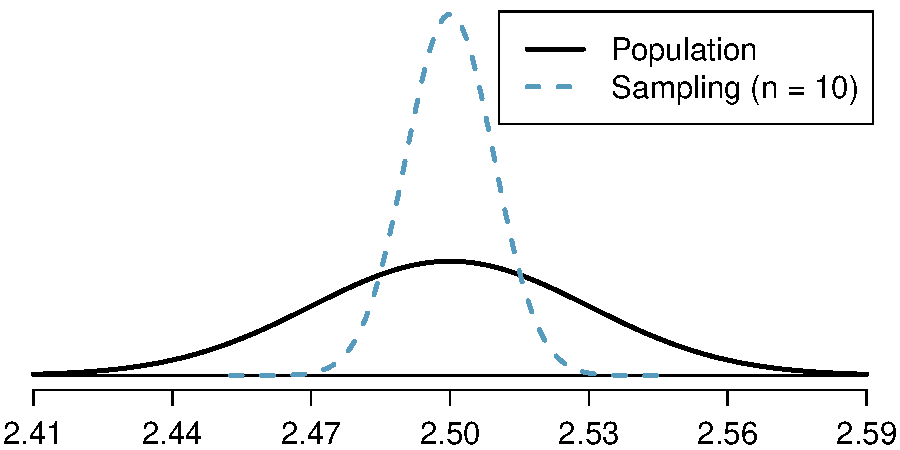
\includegraphics[width=0.48\textwidth]{ch_inference_foundations/figures/eoce/penny_weights/penny_weights_sketch.pdf}
\end{center}
(e)~We could not estimate (a) without a nearly normal population distribution. We also could not estimate (c) since the sample size is not sufficient to yield a nearly normal sampling distribution if the population distribution is not nearly normal.}

% 41

\eocesol{(a)~We cannot use the normal model for this calculation, but we can use the 
histogram. About 500 songs are shown to be longer than 5 minutes, so the 
probability is about $500/3000 = 0.167$.
(b)~Two different answers are reasonable. $^{Option~1}$Since the population 
distribution is only slightly skewed to the right, even a small sample size will 
yield a nearly normal sampling distribution. We also know that the songs are 
sampled randomly and the sample size is less than 10\% of the population, so the 
length of one song in the sample is independent of another.  We are looking for 
the probability that the total length of 15 songs is more than 60 minutes, which 
means that the average song should last at least $60/15 = 4$ minutes. Using 
$SD_{\bar{x}}=1.63/\sqrt{15}$, $Z=1.31$ $\to$ 0.0951. $^{Option~2}$Since the 
population distribution is not normal, a small sample size may not be sufficient 
to yield a nearly normal sampling distribution. Therefore, we cannot estimate 
the probability using the tools we have learned so far.
(c)~We can now be confident that the conditions are satisfied. 
$Z = 0.92$ $\to$ 0.1788.}

% 43

\eocesol{(a)~$H_0: \mu_{2009} = \mu_{2004}$. $H_A: \mu_{2009} \ne \mu_{2004}$.
(b)~$\bar{x}_{2009} - \bar{x}_{2004} = -3.6$ spam emails per day.
(c)~The null hypothesis was not rejected, and the data do not provide convincing 
evidence that the true average number of spam emails per day in years 2004 and 
2009 are different. The observed difference is about what we might expect from 
sampling variability alone.
(d)~Yes, since the hypothesis of no difference was not rejected in part~(c).}

% 45

\eocesol{(a)~$H_0: p_{2009} = p_{2004}$.  $H_A: p_{2009} \ne p_{2004}$.
(b)~-7\%.
(c)~The null hypothesis was rejected. The data provide strong evidence that the 
true proportion of those who once a month or less frequently delete their spam 
email was higher in 2004 than in 2009. The difference is so large that it cannot 
easily be explained as being due to chance.
(d)~No, since the null difference, 0, was rejected in part (c).}

% 47

\eocesol{True. If the sample size is large, then the standard error will be small, 
meaning even relatively small differences between the null value and point 
estimate can be statistically significant.}


\end{multicols}

\textC{\newpage}













\eocesolch{Inference for numerical data}

%%%%%%%%%%%%%%%%%%%%%%%%%%%%%

\begin{multicols}{2}

% 1
\eocesol{(a)~$df=6-1=5$, $t_{5}^{\star} = 2.02$ (column with two tails of 0.10, row with $df=5$).
(b)~$df=21-1=20$, $t_{20}^{\star} = 2.53$ (column with two tails of 0.02, row with $df=20$).
(c)~$df=28$, $t_{28}^{\star} = 2.05$.
(d)~$df=11$, $t_{11}^{\star} = 3.11$.}

% 3
\eocesol{(a)~between 0.025 and 0.05
(b)~less than 0.005
(c)~greater than 0.2
(d)~between 0.01 and 0.025}

% 5
\eocesol{The mean is the midpoint: $\bar{x} = 20$. Identify the margin of error: $ME = 1.015$, then use $t^{\star}_{35} = 2.03$ and $SE=s/\sqrt{n}$ in the formula for margin of error to identify $s = 3$.}

% 7
\eocesol{(a)~$H_0$: $\mu = 8$ (New Yorkers sleep 8 hrs per night on average.) $H_A$: $\mu < 8$ (New Yorkers sleep less than 8 hrs per night on average.)
(b)~Independence: The sample is random and from less than 10\% of New Yorkers. The sample is small, so we will use a $t$-distribution. For this size sample, slight skew is acceptable, and the min/max suggest there is not much skew in the data. $T = -1.75$. $df=25-1=24$.
(c)~$0.025 <$ p-value $<0.05$. If in fact the true population mean of the amount New Yorkers sleep per night was 8 hours, the probability of getting a random sample of 25 New Yorkers where the average amount of sleep is 7.73 hrs per night or less is between 0.025 and 0.05.
(d)~Since p-value $<$ 0.05, reject $H_0$. The data provide strong evidence that New Yorkers sleep less than 8 hours per night on average.
(e)~No, as we rejected $H_0$.}

% 9
\eocesol{$t^{\star}_{19}$ is 1.73 for a one-tail. We want the lower tail, so set -1.73 equal to the T-score, then solve for $\bar{x}$: 56.91.}

% 11
\eocesol{(a)~We will conduct a 1-sample $t$-test. $H_0$: $\mu = 5$. $H_A$: $\mu < 5$. We'll use $\alpha = 0.05$. This is a random sample, so the observations are independent. To proceed, we assume the distribution of years of piano lessons is approximately normal. $SE = 2.2 / \sqrt{20} = 0.4919$. The test statistic is $T = (4.6 - 5) / SE = -0.81$. $df = 20 - 1 = 19$. The one-tail p-value is about 0.21, which is bigger than $\alpha = 0.05$, so we do not reject $H_0$. That is, we do not have sufficiently strong evidence to reject Georgianna's claim. \\
(b)~Using $SE = 0.4919$ and $t_{df = 19}^{\star} = 2.093$, the confidence interval is (3.57, 5.63). We are 95\% confident that the average number of years a child takes piano lessons in this city is 3.57 to 5.63 years. \\
(c)~They agree, since we did not reject the null hypothesis and the null value of 5 was in the $t$-interval.}

% 13
\eocesol{If the sample is large, then the margin of error will be about $1.96 \times 100 / \sqrt{n}$. We want this value to be less than 10, which leads to $n \geq 384.16$, meaning we need a sample size of at least 385 (round up for sample size calculations!).}

% 15
\eocesol{(a)~Two-sided, we are evaluating a difference, not in a particular direction.
(b)~Paired, data are recorded in the same cities at two different time points. The temperature in a city at one point is not independent of the temperature in the same city at another time point.
(c)~$t$-test, sample is small and population standard deviation is unknown.
}

% 17
\eocesol{(a)~Since it�s the same students at the beginning and the end of the semester, there is a pairing between the datasets, for a given student their beginning and end of semester grades are dependent.
(b)~Since the subjects were sampled randomly, each observation in the men�s group does not have a special correspondence with exactly one observation in the other (women�s) group.
(c)~Since it�s the same subjects at the beginning and the end of the study, there is a pairing between the datasets, for a subject student their beginning and end of semester artery thickness are dependent.
(d)~Since it�s the same subjects at the beginning and the end of the study, there is a pairing between the datasets, for a subject student their beginning and end of semester weights are dependent.}

\textC{
\end{multicols}
\newpage
\begin{multicols}{2}
}

% 19
\eocesol{(a)~For each observation in one data set, there is exactly one specially-corresponding observation in the other data set for the same geographic location. The data are paired.
(b)~$H_0: \mu_{diff} = 0$ (There is no difference in average daily high temperature between January 1, 1968 and January 1, 2008 in the continental US.) $H_A: \mu_{diff} > 0$ (Average daily high temperature in January 1, 1968 was lower than average daily high temperature in January, 2008 in the continental US.) If you chose a two-sided test, that would also be acceptable. If this is the case, note that your p-value will be a little bigger than what is reported here in part~(d).
(c)~Independence: locations are random and represent less than 10\% of all possible locations in the US. The sample size is at least 30. We are not given the distribution to check the skew. In practice, we would ask to see the data to check this condition, but here we will move forward under the assumption that it is not strongly skewed.
(d)~$Z=1.60$ $\to$ p-value $=0.0548$.
(e)~Since the p-value $> \alpha$ (since not given use 0.05), fail to reject $H_0$. The data do not provide strong evidence of temperature warming in the continental US. However it should be noted that the p-value is very close to 0.05.
(f)~Type 2, since we may have incorrectly failed to reject $H_0$. There may be an increase, but we were unable to detect it.
(g)~Yes, since we failed to reject $H_0$, which had a null value of 0.}

% 21
\eocesol{(a)~(-0.03, 2.23).
(b)~We are 90\% confident that the average daily high on January 1, 2008 in the continental US was 0.03 degrees lower to 2.23 degrees higher than the average daily high on January 1, 1968.
(c)~No, since 0 is included in the interval.}

% 23
\eocesol{(a)~Each of the 36 mothers is related to exactly one of the 36 fathers (and vice-versa), so there is a special correspondence between the mothers and fathers.
(b)~$H_0: \mu_{diff} = 0$. $H_A: \mu_{diff} \ne 0$. Independence: random sample from less than 10\% of population. Sample size of at least 30. The skew of the differences is, at worst, slight. $Z = 2.72$ $\to$ p-value $= 0.0066$. Since p-value $<$ 0.05, reject $H_0$. The data provide strong evidence that the average IQ scores of mothers and fathers of gifted children are different, and the data indicate that mothers' scores are higher than fathers' scores for the parents of gifted children.}

% 25
\eocesol{No, he should not move forward with the test since the distributions of total personal income are very strongly skewed. When sample sizes are large, we can be a bit lenient with skew. However, such strong skew observed in this exercise would require somewhat large sample sizes, somewhat higher than~30.}

% 27
\eocesol{(a)~These data are paired. For example, the Friday the 13th in say, September 1991, would probably be more similar to the Friday the 6th in September 1991 than to Friday the 6th in another month or year.
(b)~Let $\mu_{diff} = \mu_{sixth} - \mu_{thirteenth}$. $H_0: \mu_{diff} = 0$. $H_A: \mu_{diff} \ne 0$.
(c)~Independence: The months selected are not random. However, if we think these dates are roughly equivalent to a simple random sample of all such Friday 6th/13th date pairs, then independence is reasonable. To proceed, we must make this strong assumption, though we should note this assumption in any reported results. With fewer than 10 observations, we would need to use the $t$-distribution to model the sample mean. The normal probability plot of the differences shows an approximately straight line. There isn't a clear reason why this distribution would be skewed, and since the normal quantile plot looks reasonable, we can mark this condition as reasonably satisfied.
(d)~$T = 4.94$ for $df=10-1=9$ $\to$ p-value $<0.01$.
(e)~Since p-value $<$ 0.05, reject $H_0$. The data provide strong evidence that the average number of cars at the intersection is higher on Friday the 6$^{\text{th}}$ than on Friday the 13$^{\text{th}}$. (We might believe this intersection is representative of all roads, i.e. there is higher traffic on Friday the 6$^{\text{th}}$ relative to Friday the 13$^{\text{th}}$. However, we should be cautious of the required assumption for such a generalization.)
(f)~If the average number of cars passing the intersection actually was the same on Friday the 6$^{\text{th}}$ and $13^{th}$, then the probability that we would observe a test statistic so far from zero is less than 0.01.
(g)~We might have made a Type 1 error, i.e. incorrectly rejected the null hypothesis.}

\textC{
\end{multicols}
\newpage
\begin{multicols}{2}
}

% 29
\eocesol{(a)~$H_0: \mu_{diff} = 0$. $H_A: \mu_{diff} \ne 0$. $T=-2.71$. $df=5$. $0.02<$ p-value $<0.05$. Since p-value $<$ 0.05, reject $H_0$. The data provide strong evidence that the average number of traffic accident related emergency room admissions are different between Friday the 6$^{\text{th}}$ and Friday the 13$^{\text{th}}$. Furthermore, the data indicate that the direction of that difference is that accidents are lower on Friday the $6^{th}$ relative to Friday the 13$^{\text{th}}$.
(b)~(-6.49, -0.17).
(c)~This is an observational study, not an experiment, so we cannot so easily infer a causal intervention implied by this statement. It is true that there is a difference. However, for example, this does not mean that a responsible adult going out on Friday the $13^{th}$ has a higher chance of harm than on any other night.}

% 31
\eocesol{(a)~Chicken fed linseed weighed an average of 218.75 grams while those fed horsebean weighed an average of 160.20 grams. Both distributions are relatively symmetric with no apparent outliers. There is more variability in the weights of chicken fed linseed.
(b)~$H_0: \mu_{ls} = \mu_{hb}$. $H_A: \mu_{ls} \ne \mu_{hb}$. We leave the conditions to you to consider. $T=3.02$, $df = min(11, 9) = 9$ $\to$ $0.01<$ p-value $<0.02$. Since p-value $<$ 0.05, reject $H_0$. The data provide strong evidence that there is a significant difference between the average weights of chickens that were fed linseed and horsebean.
(c)~Type 1, since we rejected $H_0$.
(d)~Yes, since p-value $>$ 0.01, we would have failed to reject~$H_0$.}

% 33
\eocesol{$H_0: \mu_C = \mu_S$. $H_A: \mu_C \ne \mu_S$. $T = 3.27$, $df=11$ $\to$ p-value $<0.01$. Since p-value $< 0.05$, reject $H_0$. The data provide strong evidence that the average weight of chickens that were fed casein is different than the average weight of chickens that were fed soybean (with weights from casein being higher). Since this is a randomized experiment, the observed difference can be attributed to the diet.}

% 35
\eocesol{$H_0: \mu_{T} = \mu_{C}$. $H_A: \mu_{T} \ne \mu_{C}$. $T=2.24$, $df=21$ $\to$ $0.02<$ p-value $<0.05$. Since p-value $<$ 0.05, reject $H_0$. The data provide strong evidence that the average food consumption by the patients in the treatment and control groups are different. Furthermore, the data indicate patients in the distracted eating (treatment) group consume more food than patients in the control group.}

% 37
\eocesol{Let $\mu_{diff} = \mu_{pre} - \mu_{post}$. $H_0: \mu_{diff} = 0$: Treatment has no effect. $H_A: \mu_{diff} > 0$: Treatment is effective in reducing Pd T scores, the average pre-treatment score is higher than the average post-treatment score. Note that the reported values are pre minus post, so we are looking for a positive difference, which would correspond to a reduction in the psychopathic deviant T score. Conditions are checked as follows. Independence: The subjects are randomly assigned to treatments, so the patients in each group are independent. All three sample sizes are smaller than 30, so we use $t$-tests. Distributions of differences are somewhat skewed. The sample sizes are small, so we cannot reliably relax this assumption. (We will proceed, but we would not report the results of this specific analysis, at least for treatment group 1.) For all three groups: $df=13$. $T_1= 1.89$ ($0.025<$ p-value $<0.05$), $T_2=1.35$ (p-value = 0.10), $T_3 = -1.40$ (p-value $>0.10$). The only significant test reduction is found in Treatment 1, however, we had earlier noted that this result might not be reliable due to the skew in the distribution. Note that the calculation of the p-value for Treatment 3 was unnecessary: the sample mean indicated a increase in Pd T scores under this treatment (as opposed to a decrease, which was the result of interest). That is, we could tell without formally completing the hypothesis test that the p-value would be large for this treatment group.}

% 39
\eocesol{Alternative.}

% 41
\eocesol{$H_0$: $\mu_1 = \mu_2 = \cdots = \mu_6$. $H_A$: The average weight varies across some (or all) groups. Independence: Chicks are randomly assigned to feed types (presumably kept separate from one another), therefore independence of observations is reasonable. Approx. normal: the distributions of weights within each feed type appear to be fairly symmetric. Constant variance: Based on the side-by-side box plots, the constant variance assumption appears to be reasonable. There are differences in the actual computed standard deviations, but these might be due to chance as these are quite small samples. $F_{5,65} = 15.36$ and the p-value is approximately 0. With such a small p-value, we reject $H_0$. The data provide convincing evidence that the average weight of chicks varies across some (or all) feed supplement groups.}

\textC{
\end{multicols}
\newpage
\begin{multicols}{2}
}

% 43
\eocesol{(a)~$H_0$: The population mean of MET for each group is equal to the others. $H_A$: At least one pair of means is different.
(b)~Independence: We don't have any information on how the data were collected, so we cannot assess independence. To proceed, we must assume the subjects in each group are independent. In practice, we would inquire for more details. Approx. normal: The data are bound below by zero and the standard deviations are larger than the means, indicating very strong strong skew. However, since the sample sizes are extremely large, even extreme skew is acceptable. Constant variance: This condition is sufficiently met, as the standard deviations are reasonably consistent across groups.
(c)~See below, with the last column omitted:\\[-2mm]
\begin{adjustwidth}{-4em}{-4em}
{\tiny
\begin{center}
\renewcommand{\arraystretch}{1.25}
\begin{tabular}{lrrrr}
  \hline
            & Df    & Sum Sq        & Mean Sq   & F value \\ 
  \hline
coffee      & {\textcolor{oiB}{{\scriptsize 4}}}     & {\textcolor{oiB}{{\scriptsize 10508}}}       & {\textcolor{oiB}{{\scriptsize 2627}}}             & {\textcolor{oiB}{{\scriptsize 5.2}}} \\ 
Residuals       & {\textcolor{oiB}{{\scriptsize 50734}}} & 25564819     & {\textcolor{oiB}{{\scriptsize  504}}}         &  \\ 
   \hline
Total           & {\textcolor{oiB}{{\scriptsize 50738}}} & 25575327 \\
\hline
\end{tabular}
\end{center}
}
\end{adjustwidth} \vspace{1mm}
(d)~Since p-value is very small, reject $H_0$. The data provide convincing evidence that the average MET differs between at least one pair of groups.}

% 45
\eocesol{(a)~$H_0$: Average GPA is the same for all majors. $H_A$: At least one pair of means are different.
(b)~Since p-value $>$ 0.05, fail to reject $H_0$. The data do not provide convincing evidence of a difference between the average GPAs across three groups of majors.
(c)~The total degrees of freedom is $195 + 2 = 197$, so the sample size is $197+1=198$.}

% 47
\eocesol{(a)~False. As the number of groups increases, so does the number of comparisons and hence the modified significance level decreases.
(b)~True.
(c)~True.
(d)~False. We need observations to be independent regardless of sample size.}

% 49
\eocesol{(a)~$H_0$: Average score difference is the same for all treatments. $H_A$: At least one pair of means are different.
(b)~We should check conditions. If we look back to the earlier exercise, we will see that the patients were randomized, so independence is satisfied. There are some minor concerns about skew, especially with the third group, though this may be acceptable. The standard deviations across the groups are reasonably similar. Since the p-value is less than 0.05, reject $H_0$. The data provide convincing evidence of a difference between the average reduction in score among treatments.
(c)~We determined that at least two means are different in part (b), so we now conduct $K=3\times2/2=3$ pairwise $t$-tests that each use $\alpha=0.05/3 = 0.0167$ for a significance level. Use the following hypotheses for each pairwise test. $H_0$: The two means are equal. $H_A$: The two means are different. The sample sizes are equal and we use the pooled SD, so we can compute $SE=3.7$ with the pooled $df=39$. The p-value only for Trmt 1 vs. Trmt 3 may be statistically significant: $0.01<$ p-value $<0.02$. Since we cannot tell, we should use a computer to get the p-value, 0.015, which is statistically significant for the adjusted significance level. That is, we have identified Treatment 1 and Treatment 3 as having different effects. Checking the other two comparisons, the differences are not statistically significant.}

\end{multicols}

%%%%%%%%%%%%%%%%%%%%%%%%%%%%%

% Chp 6
\eocesolch{Inference for categorical data}

%%%%%%%%%%%%%%%%%%%%%%%%%%%%%

\begin{multicols}{2}

% 1
\eocesol{(a)~False. Doesn't satisfy success-failure condition.
(b)~True. The success-failure condition is not satisfied. In most samples we would expect $\hat{p}$ to be close to 0.08, the true population proportion. While $\hat{p}$ can be much above 0.08, it is bound below by 0, suggesting it would take on a right skewed shape. Plotting the sampling distribution would confirm this suspicion.
(c)~False. $SE_{\hat{p}} = 0.0243$, and $\hat{p} = 0.12$ is only $\frac{0.12 - 0.08}{0.0243} = 1.65$ SEs away from the mean, which would not be considered unusual.
(d)~True. $\hat{p}=0.12$ is 2.32 standard errors away from the mean, which is often considered unusual.
(e)~False. Decreases the SE by a factor of $1/\sqrt{2}$.}

% 3
\eocesol{(a)~True. See the reasoning of 6.1(b).
(b)~True. We take the square root of the sample size in the SE formula.
(c)~True. The independence and success-failure conditions are satisfied.
(d)~True. The independence and success-failure conditions are satisfied.}

% 5
\eocesol{(a)~False. A confidence interval is constructed to estimate the population proportion, not the sample proportion.
(b)~True. 95\% CI: $70\%\ \pm\ 8\%$.
(c)~True. By the definition of the confidence level.
(d)~True. Quadrupling the sample size decreases the SE and ME by a factor of $1/\sqrt{4}$.
(e)~True. The 95\% CI is entirely above 50\%.}

\textC{
\end{multicols}
\newpage
\begin{multicols}{2}
}

% 7
\eocesol{With a random sample from $<10\%$ of the population, independence is satisfied. The success-failure condition is also satisfied. $ME = z^{\star} \sqrt{ \frac{\hat{p} (1-\hat{p})} {n} } = 1.96 \sqrt{ \frac{0.56 \times  0.44}{600} }= 0.0397 \approx 4\%$}

% 9
\eocesol{(a)~Proportion of graduates from this university who found a job within one year of graduating. $\hat{p} = 348/400 = 0.87$.
(b)~This is a random sample from less than 10\% of the population, so the observations are independent. Success-failure condition is satisfied: 348 successes, 52 failures, both well above~10.
(c)~(0.8371, 0.9029). We are 95\% confident that approximately 84\% to 90\% of graduates from this university found a job within one year of completing their undergraduate degree.
(d)~95\% of such random samples would produce a 95\% confidence interval that includes the true proportion of students at this university who found a job within one year of graduating from college.
(e)~(0.8267, 0.9133). Similar interpretation as before.
(f)~99\% CI is wider, as we are more confident that the true proportion is within the interval and so need to cover a wider range.}

% 11
\eocesol{(a)~No. The sample only represents students who took the SAT, and this was also an online survey.
(b)~(0.5289, 0.5711). We are 90\% confident that 53\% to 57\% of high school seniors who took the SAT are fairly certain that they will participate in a study abroad program in college.
(c)~90\% of such random samples would produce a 90\% confidence interval that includes the true proportion.
(d)~Yes. The interval lies entirely above 50\%.}

% 13
\eocesol{(a)~This is an appropriate setting for a hypothesis test. $H_0: p = 0.50$. $H_A:  p > 0.50$. Both independence and the success-failure condition are satisfied. $Z=1.12$ $\to$ p-value $= 0.1314$. Since the p-value $> \alpha=0.05$, we fail to reject $H_0$. The data do not provide strong evidence in favor of the claim.
(b)~Yes, since we did not reject $H_0$ in part~(a).}

% 15
\eocesol{(a)~$H_0: p = 0.38$. $H_A: p \ne 0.38$. Independence (random sample, $<10\%$ of population) and the success-failure condition are satisfied. $Z=-20.5$ $\to$ p-value $\approx 0$. Since the p-value is very small, we reject $H_0$. The data provide strong evidence that the proportion of Americans who only use their cell phones to access the internet is different than the Chinese proportion of 38\%, and the data indicate that the proportion is lower in the US.
(b)~If in fact 38\% of Americans used their cell phones as a primary access point to the internet, the probability of obtaining a random sample of 2,254 Americans where 17\% or less or 59\% or more use their only their cell phones to access the internet would be approximately 0.
(c)~(0.1545, 0.1855). We are 95\% confident that approximately 15.5\% to 18.6\% of all Americans primarily use their cell phones to browse the internet.}

% 17
\eocesol{(a)~$H_0: p = 0.5$. $H_A: p > 0.5$. Independence (random sample, $<10\%$ of population) is satisfied, as is the success-failure conditions (using $p_0 = 0.5$, we expect 40 successes and 40 failures). $Z = 2.91$ $\to$ p-value $= 0.0018$. Since the p-value $< 0.05$, we reject the null hypothesis. The data provide strong evidence that the rate of correctly identifying a soda for these people is significantly better than just by random guessing.
(b)~If in fact people cannot tell the difference between diet and regular soda and they randomly guess, the probability of getting a random sample of 80 people where 53 or more identify a soda correctly would be 0.0018.}

% 19
\eocesol{(a)~Independence is satisfied (random sample from $<10\%$ of the population), as is the success-failure condition (40 smokers, 160 non-smokers). The 95\% CI: (0.145, 0.255). We are 95\% confident that 14.5\% to 25.5\% of all students at this university smoke.
(b)~We want $z^{\star}SE$ to be no larger than 0.02 for a 95\% confidence level. We use $z^{\star}=1.96$ and plug in the point estimate $\hat{p}=0.2$ within the SE formula: $1.96\sqrt{0.2(1-0.2)/n} \leq 0.02$. The sample size $n$ should be at least 1,537.}

% 21
\eocesol{The margin of error, which is computed as $z^{\star}SE$, must be smaller than 0.01 for a 90\% confidence level. We use $z^{\star} = 1.65$ for a 90\% confidence level, and we can use the point estimate $\hat{p}=0.52$ in the formula for $SE$. $1.65\sqrt{0.52(1-0.52)/n} \leq 0.01$. Therefore, the sample size $n$ must be at least 6,796.}

% 23
\eocesol{This is not a randomized experiment, and it is unclear whether people would be affected by the behavior of their peers. That is, independence may not hold. Additionally, there are only 5 interventions under the provocative scenario, so the success-failure condition does not hold. Even if we consider a hypothesis test where we pool the proportions, the success-failure condition will not be satisfied. Since one condition is questionable and the other is not satisfied, the difference in sample proportions will not follow a nearly normal distribution.}

\textC{
\end{multicols}
\newpage
\begin{multicols}{2}
}

% 25
\eocesol{(a)~False. The entire confidence interval is above 0.
(b)~True.
(c)~True.
(d)~True.
(e)~False. It is simply the negated and reordered values: \mbox{(-0.06,-0.02)}.}

% 27
\eocesol{(a)~(0.23, 0.33). We are 95\% confident that the proportion of Democrats who support the plan is 23\% to 33\% higher than the proportion of Independents who do.
(b)~True.}

% 29
\eocesol{(a)~College grads: 23.7\%. Non-college grads: 33.7\%.
(b)~Let $p_{CG}$ and $p_{NCG}$ represent the proportion of college graduates and non-college graduates who responded ``do not know". $H_0: p_{CG} = p_{NCG}$. $H_A: p_{CG} \ne p_{NCG}$. Independence is satisfied (random sample, $<10\%$ of the population), and the success-failure condition, which we would check using the pooled proportion ($\hat{p} = 235/827 = 0.284$), is also satisfied. $Z=-3.18$ $\to$ p-value = 0.0014. Since the p-value is very small, we reject $H_0$. The data provide strong evidence that the proportion of college graduates who do not have an opinion on this issue is different than that of non-college graduates. The data also indicate that fewer college grads say they ``do not know'' than non-college grads (i.e. the data indicate the direction after we reject $H_0$).}

% 31
\eocesol{(a)~College grads: 35.2\%. Non-college grads: 33.9\%.
(b)~Let $p_{CG}$ and $p_{NCG}$ represent the proportion of college graduates and non-college grads who support offshore drilling. $H_0: p_{CG} = p_{NCG}$. $H_A: p_{CG} \ne p_{NCG}$. Independence is satisfied (random sample, $<10\%$ of the population), and the success-failure condition, which we would check using the pooled proportion ($\hat{p} = 286/827 = 0.346$), is also satisfied. $Z = 0.39$ $\to$ p-value $=0.6966$. Since the p-value $> \alpha$ (0.05), we fail to reject $H_0$. The data do not provide strong evidence of a difference between the proportions of college graduates and non-college graduates who support off-shore drilling in California.}

% 33
\eocesol{Subscript $_C$ means control group. Subscript $_T$ means truck drivers. $H_0: p_C = p_T$. $H_A: p _C \ne p_T$. Independence is satisfied (random samples, $<10\%$ of the population), as is the success-failure condition, which we would check using the pooled proportion ($\hat{p} = 70/495 = 0.141$). $Z = -1.58$ $\to$ p-value $=0.1164$. Since the p-value is high, we fail to reject $H_0$. The data do not provide strong evidence that the rates of sleep deprivation are different for non-transportation workers and truck drivers.}

% 35
\eocesol{(a)~Summary of the study:
\begin{center}\scriptsize
\begin{tabular}{l l c c c}
                                &           & \multicolumn{2}{c}{\textit{Virol. failure}}   &       \\
\cline{3-4}
                                &           & Yes       & No        & Total \\
\cline{2-5}
\multirow{2}{*}{\textit{Treatment}}     & Nevaripine    & 26            & 94        & 120   \\
                                & Lopinavir & 10            & 110   & 120   \\
\cline{2-5}
                                & Total     & 36            & 204   & 240
\end{tabular}
\end{center}
(b)~$H_0: p_N = p_L$. There is no difference in virologic failure rates between the Nevaripine and Lopinavir groups. $H_A: p_N \ne p_L$. There is some difference in virologic failure rates between the Nevaripine and Lopinavir groups.
(c)~Random assignment was used, so the observations in each group are independent. If the patients in the study are representative of those in the general population (something impossible to check with the given information), then we can also confidently generalize the findings to the population. The success-failure condition, which we would check using the pooled proportion ($\hat{p} = 36/240 = 0.15$), is satisfied. $Z=3.04$ $\to$ p-value $=0.0024$. Since the p-value is low, we reject $H_0$. There is strong evidence of a difference in virologic failure rates between the Nevaripine and Lopinavir groups do not appear to be independent.}

% 37
\eocesol{No. The samples at the beginning and at the end of the semester are not independent since the survey is conducted on the same students.}

% 39
\eocesol{(a)~False. The chi-square distribution has one parameter called degrees of freedom.
(b)~True.
(c)~True.
(d)~False. As the degrees of freedom increases, the shape of the chi-square distribution becomes more symmetric.}

% 41
\eocesol{(a)~$H_0$: The distribution of the format of the book used by the students follows the professor's predictions. $H_A$: The distribution of the format of the book used by the students does not follow the professor's predictions.
(b)~$E_{hard~copy} = 126 \times  0.60 = 75.6$. $E_{print} = 126 \times  0.25 = 31.5$. $E_{online} = 126 \times  0.15 = 18.9$.
(c)~Independence:  The sample is not random. However, if the professor has reason to believe that the proportions are stable from one term to the next and students are not affecting each other's study habits, independence is probably reasonable. Sample size: All expected counts are at least 5.
(d)~$\chi^2 = 2.32$, $df=2$, p-value $> 0.3$.
(e)~Since the p-value is large, we fail to reject $H_0$. The data do not provide strong evidence indicating the professor's predictions were statistically inaccurate.}

\textC{
\end{multicols}
\newpage
\begin{multicols}{2}
}

% 43
\eocesol{Use a chi-squared goodness of fit test.
$H_0$: Each option is equally likely.
$H_A$: Some options are preferred over others.
Total sample size: 99.
Expected counts: (1/3) * 99 = 33 for each option. These are all above 5, so conditions are satisfied.
$df = 3 - 1 = 2$ and $\chi^2 = \frac{(43 - 33)^2}{33} + \frac{(21 - 33)^2}{33} + \frac{(35 - 33)^2}{33} = 7.52 \rightarrow 0.02 <$ p-value $< 0.05$. Since the p-value is less than 5\%, we reject $H_0$. The data provide convincing evidence that some options are preferred over others.}

% 45
\eocesol{(a). Two-way table:
\begin{center}\scriptsize
\begin{tabular}{l l c c c}
& \multicolumn{2}{c}{\textit{Quit}} &       \\
\cline{2-3}
\textit{Treatment}      & Yes       & No        & Total \\
\hline
Patch + support group   & 40            & 110   & 150   \\
Only patch          & 30            & 120   & 150   \\
\cline{1-4}
Total               & 70            & 230   & 300 \\
\cline{1-4}
\end{tabular}
\end{center}
(b-i)~$E_{row_1, col_1} = \frac{(row~1~total)\times(col~1~total)}{table~total} = \frac{150 \times  70}{300} = 35$. This is lower than the observed value.
(b-ii)~$E_{row_2, col_2} = \frac{(row~2~total)\times(col~2~total)}{table~total} = \frac{150 \times  230}{300} = 115$. This is lower than the observed value.}

% 47
\eocesol{$H_0$: The opinion of college grads and non-grads is not different on the topic of drilling for oil and natural gas off the coast of California. $H_A$: Opinions regarding the drilling for oil and natural gas off the coast of California has an association with earning a college degree.
\begin{align*}
&E_{row~1, col~1} = 151.5 && E_{row~1, col~2} = 134.5 \\
&E_{row~2, col~1} = 162.1 && E_{row~2, col~2} = 143.9 \\
&E_{row~3, col~1} = 124.5 && E_{row~3, col~2} = 110.5
\end{align*}
Independence: The samples are both random, unrelated, and from less than 10\% of the population, so independence between observations is reasonable. Sample size: All expected counts are at least 5.
$\chi^2 = 11.47$, $df = 2$ $\to$ $0.001<$ p-value $<0.005$.
Since the p-value $< \alpha$, we reject $H_0$.  There is strong evidence that there is an association between support for off-shore drilling and having a college degree.}

% 49
\eocesol{(a)~$H_0$:~The age of Los Angeles residents is independent of shipping carrier preference variable. $H_A$:~The age of Los Angeles residents is associated with the shipping carrier preference variable. (b)~The conditions are not satisfied since some expected counts are below~5.}

% 51
\eocesol{(a)~$H_0: p = 0.69$. $H_A: p \ne 0.69$.
(b)~$\hat{p} = \frac{17}{30} = 0.57$.
(c)~The success-failure condition is not satisfied; note that it is appropriate to use the null value ($p_0 = 0.69$) to compute the expected number of successes and failures.
(d)~Answers may vary. Each student can be represented with a card. Take 100 cards, 69 black cards representing those who follow the news about Egypt and 31 red cards representing those who do not. Shuffle the cards and draw with replacement (shuffling each time in between draws) 30 cards representing the 30 high school students. Calculate the proportion of black cards in this sample, $\hat{p}_{sim}$, i.e. the proportion of those who follow the news in the simulation. Repeat this many times (e.g. 10,000 times) and plot the resulting sample proportions. The p-value will be two times the proportion of simulations where $\hat{p}_{sim} \le 0.57$. (Note: we would generally use a computer to perform these simulations.)
(e)~The p-value is about $0.001 + 0.005 + 0.020 + 0.035 + 0.075 = 0.136$, meaning the two-sided p-value is about 0.272. Your p-value may vary slightly since it is based on a visual estimate. Since the p-value is greater than 0.05, we fail to reject $H_0$. The data do not provide strong evidence that the proportion of high school students who followed the news about Egypt is different than the proportion of American adults who did.}

\textC{
\end{multicols}
\newpage
\begin{multicols}{2}
}

% 53
\eocesol{The subscript $_{pr}$ corresponds to provocative and $_{con}$ to conservative.
(a)~$H_0: p_{pr} = p_{con}$. $H_A: p_{pr} \ne p_{con}$.
(b)~-0.35.
(c)~The left tail for the p-value is calculated by adding up the two left bins: $0.005+0.015=0.02$. Doubling the one tail, the p-value is 0.04. (Students may have approximate results, and a small number of students may have a p-value of about 0.05.) Since the p-value is low, we reject $H_0$. The data provide strong evidence that people react differently under the two scenarios.}

\end{multicols}

\eocesolch{Multiple and logistic regression}

\begin{multicols}{2}

% 1
\eocesol{(a)~$\widehat{baby\_\hspace{0.3mm}weight} = 123.05 - 8.94 \times smoke$
(b)~The estimated body weight of babies born to smoking mothers is 8.94 ounces lower than babies born to non-smoking mothers.  Smoker: $123.05 - 8.94 \times 1 = 114.11$ ounces. Non-smoker: $123.05 - 8.94 \times 0 = 123.05$ ounces.
(c)~$H_0$: $\beta_1 = 0$. $H_A$: $\beta_1 \ne 0$. $T= -8.65$, and the p-value is approximately 0. Since the p-value is very small, we reject $H_0$. The data provide strong evidence that the true slope parameter is different than 0 and that there is an association between birth weight and smoking. Furthermore, having rejected $H_0$, we can conclude that smoking is associated with lower birth weights.}

% 3
\eocesol{(a)~$\widehat{baby\_\hspace{0.3mm}weight} = -80.41 + 0.44 \times gestation - 3.33 \times parity - 0.01 \times age + 1.15 \times height + 0.05 \times weight - 8.40 \times smoke$.
(b)~$\beta_{gestation}$: The model predicts a 0.44 ounce increase in the birth weight of the baby for each additional day of pregnancy, all else held constant.  $\beta_{age}$: The model predicts a 0.01 ounce decrease in the birth weight of the baby for each additional year in mother's age, all else held constant. 
(c)~Parity might be correlated with one of the other variables in the model, which complicates model estimation.
(d)~$\widehat{baby\_\hspace{0.3mm}weight} = 120.58$.
$e = 120 - 120.58 = -0.58$. The model over-predicts this baby's birth weight.
(e)~$R^2 = 0.2504$. $R_{adj}^2 = 0.2468$.}

% 5
\eocesol{(a)~(-0.32, 0.16). We are 95\% confident that male students on average have GPAs 0.32 points lower to 0.16 points higher than females when controlling for the other variables in the model.
(b)~Yes, since the p-value is larger than 0.05 in all cases (not including the intercept).}

% 7
\eocesol{Strictly speaking, remove age. However the adjusted R-squared values for the full model and the model excluding age as a predictor are so close that not removing age would not result in a substantial amount of predictive power.}

% 9
\eocesol{Based on the p-value alone, either gestation or smoke should be added to the model first. However, since the adjusted $R^2$ for the model with gestation is higher, it would be preferable to add gestation in the first step of the forward-selection algorithm. (Other explanations are possible. For instance, it would be reasonable to only use the adjusted $R^2$.)}

% 11
\eocesol{She should use p-value selection since she is interested in finding out about significant
predictors, and not interested in making a precise prediction.}

% 13
\eocesol{Nearly normal residuals: The normal probability plot shows a nearly normal distribution of the residuals, however, there are some minor irregularities at the tails. With a data set so large, these would not be a concern. \\ Constant variability of residuals: The scatterplot of the residuals versus the fitted values does not show any overall structure. However, values that have very low or very high fitted values appear to also have somewhat larger outliers. In addition, the residuals do appear to have constant variability between the two parity and smoking status groups, though these items are relatively minor. \\ Independent residuals: The scatterplot of residuals versus the order of data collection shows a random scatter, suggesting that there is no apparent structures related to the order the data were collected. \\ Linear relationships between the response variable and numerical explanatory variables: The residuals vs. height and weight of mother are randomly distributed around 0. The residuals vs. length of gestation plot also does not show any clear or strong remaining structures, with the possible exception of very short or long gestations. The rest of the residuals do appear to be randomly distributed around 0. \\All concerns raised here are relatively mild. There are some outliers, but there is so much data that the influence of such observations will be minor.}


\textC{
\end{multicols}
\newpage
\begin{multicols}{2}
}

% 15
\eocesol{(a)~There are a few potential outliers, e.g. on the left in the \var{total\_\hspace{0.3mm}length} variable, but nothing that will be of serious concern in a data set this large.
(b)~When coefficient estimates are sensitive to which variables are included in the model, this typically indicates that some variables are collinear. For example, a possum's gender may be related to its head length, which would explain why the coefficient (and p-value) for \var{sex\_\hspace{0.3mm}male} changed when we removed the \var{head\_\hspace{0.3mm}length} variable. Likewise, a possum's skull width is likely to be related to its head length, probably even much more closely related than the head length was to gender.}

% 17
\eocesol{(a)~The logistic model relating $\hat{p}_i$ to the predictors may be written as 
$\log\left( \frac{\hat{p}_i}{1 - \hat{p}_i} \right) = 33.5095 - 1.4207\times sex\_male_i - 0.2787 \times skull\_width_i + 0.5687 \times total\_length_i$. Only \var{total\_\hspace{0.3mm}length} has a positive association with a possum being from Victoria.
(b)~$\hat{p} = 0.0062$. While the probability is very near zero, we have not run diagnostics on the model. We might also be a little skeptical that the model will remain accurate for a possum found in a US zoo. For example, perhaps the zoo selected a possum with specific characteristics but only looked in one region. On the other hand, it is encouraging that the possum was caught in the wild. (Answers regarding the reliability of the model probability will vary.)}

\end{multicols}



\eocesolch{Multiple and logistic regression}

\begin{multicols}{2}

% 1
\eocesol{(a)~$\widehat{baby\_\hspace{0.3mm}weight} = 123.05 - 8.94 \times smoke$
(b)~The estimated body weight of babies born to smoking mothers is 8.94 ounces lower than babies born to non-smoking mothers.  Smoker: $123.05 - 8.94 \times 1 = 114.11$ ounces. Non-smoker: $123.05 - 8.94 \times 0 = 123.05$ ounces.
(c)~$H_0$: $\beta_1 = 0$. $H_A$: $\beta_1 \ne 0$. $T= -8.65$, and the p-value is approximately 0. Since the p-value is very small, we reject $H_0$. The data provide strong evidence that the true slope parameter is different than 0 and that there is an association between birth weight and smoking. Furthermore, having rejected $H_0$, we can conclude that smoking is associated with lower birth weights.}

% 3
\eocesol{(a)~$\widehat{baby\_\hspace{0.3mm}weight} = -80.41 + 0.44 \times gestation - 3.33 \times parity - 0.01 \times age + 1.15 \times height + 0.05 \times weight - 8.40 \times smoke$.
(b)~$\beta_{gestation}$: The model predicts a 0.44 ounce increase in the birth weight of the baby for each additional day of pregnancy, all else held constant.  $\beta_{age}$: The model predicts a 0.01 ounce decrease in the birth weight of the baby for each additional year in mother's age, all else held constant. 
(c)~Parity might be correlated with one of the other variables in the model, which complicates model estimation.
(d)~$\widehat{baby\_\hspace{0.3mm}weight} = 120.58$.
$e = 120 - 120.58 = -0.58$. The model over-predicts this baby's birth weight.
(e)~$R^2 = 0.2504$. $R_{adj}^2 = 0.2468$.}

% 5
\eocesol{(a)~(-0.32, 0.16). We are 95\% confident that male students on average have GPAs 0.32 points lower to 0.16 points higher than females when controlling for the other variables in the model.
(b)~Yes, since the p-value is larger than 0.05 in all cases (not including the intercept).}

% 7
\eocesol{Strictly speaking, remove age. However the adjusted R-squared values for the full model and the model excluding age as a predictor are so close that not removing age would not result in a substantial amount of predictive power.}

% 9
\eocesol{Based on the p-value alone, either gestation or smoke should be added to the model first. However, since the adjusted $R^2$ for the model with gestation is higher, it would be preferable to add gestation in the first step of the forward-selection algorithm. (Other explanations are possible. For instance, it would be reasonable to only use the adjusted $R^2$.)}

% 11
\eocesol{She should use p-value selection since she is interested in finding out about significant
predictors, and not interested in making a precise prediction.}

% 13
\eocesol{Nearly normal residuals: The normal probability plot shows a nearly normal distribution of the residuals, however, there are some minor irregularities at the tails. With a data set so large, these would not be a concern. \\ Constant variability of residuals: The scatterplot of the residuals versus the fitted values does not show any overall structure. However, values that have very low or very high fitted values appear to also have somewhat larger outliers. In addition, the residuals do appear to have constant variability between the two parity and smoking status groups, though these items are relatively minor. \\ Independent residuals: The scatterplot of residuals versus the order of data collection shows a random scatter, suggesting that there is no apparent structures related to the order the data were collected. \\ Linear relationships between the response variable and numerical explanatory variables: The residuals vs. height and weight of mother are randomly distributed around 0. The residuals vs. length of gestation plot also does not show any clear or strong remaining structures, with the possible exception of very short or long gestations. The rest of the residuals do appear to be randomly distributed around 0. \\All concerns raised here are relatively mild. There are some outliers, but there is so much data that the influence of such observations will be minor.}


\textC{\pagebreak}

% 15
\eocesol{(a)~There are a few potential outliers, e.g. on the left in the \var{total\_\hspace{0.3mm}length} variable, but nothing that will be of serious concern in a data set this large.
(b)~When coefficient estimates are sensitive to which variables are included in the model, this typically indicates that some variables are collinear. For example, a possum's gender may be related to its head length, which would explain why the coefficient (and p-value) for \var{sex\_\hspace{0.3mm}male} changed when we removed the \var{head\_\hspace{0.3mm}length} variable. Likewise, a possum's skull width is likely to be related to its head length, probably even much more closely related than the head length was to gender.}\textC{\vspace{10mm}}


% 17
\eocesol{(a)~The logistic model relating $\hat{p}_i$ to the predictors may be written as 
$\log\left( \frac{\hat{p}_i}{1 - \hat{p}_i} \right) = 33.5095 - 1.4207\times sex\_male_i - 0.2787 \times skull\_width_i + 0.5687 \times total\_length_i$. Only \var{total\_\hspace{0.3mm}length} has a positive association with a possum being from Victoria.
(b)~$\hat{p} = 0.0062$. While the probability is very near zero, we have not run diagnostics on the model. We might also be a little skeptical that the model will remain accurate for a possum found in a US zoo. For example, perhaps the zoo selected a possum with specific characteristics but only looked in one region. On the other hand, it is encouraging that the possum was caught in the wild. (Answers regarding the reliability of the model probability will vary.)}

\end{multicols}
